\pagestyle{fancy}
\rhead{\thepage}
\lhead{Introduction}
\chapter{Introduction}

With the rapid development of digital audio technolodge, people start to find out that computers are playing an increasingly important role in music. This new trend is providing unprecedented opportunities for people to create and manipulate sound. However, the flexibility of the digital technolodge is accompanied by confuse and uncertainty. As a result, thousands of new musicial forms built on computers have been created and released to the world. And it is natural to ask, what kinds of musical interfaces are taking better advantage of computers. To answer this question, researchers targeting at the better establised field of human-computer interaction \citep{Reference16}. Under the circumstance of new musical form explosion, a new community called NIME was born (see \ref{subsec: nime}).

\section{Background}
\label{sec: backgound}

\subsection{The development of NIME}
\label{subsec: nime}
% what is NIME and it's development
The New Interface for Musical Expression (NIME) is an international conference for musicians and researchers from all over the world to demonstrate their latest work on musical interface design \citep{Reference15}. It first started as a workshop at the Conference on Human Factors in Computing System (CHI) in 2001. After that, annually conferences have been held around the world. The hoster are research groups who devote themselves to interface design, human-computer interaction and computer music. The latest conference was held at Griffith University in Brisbane, Queensland, Australia in 2016.

In the last sixteen years, NIME has explored different approaches on new musical interface design. The \textit{reacTable} which was designed for live music performance on tabletop led a new trend on tangible music interface \citep{Reference17}. Many researchers shifted their attention to this new media. Toolkit such as reacTiVision was developed to detect movement of performers and allow further development to turn any surface into a musical instrument \citep{Reference18}.

The success of \textit{Smule} initiated a new era of mobile music \citep{Reference8}. After that, thousands of musical applications such as \textit{MoMu, MadPad and Magic Fiddle} which were specifically designed for mobile devices were developed \citep{Reference8.2,Reference8.3,Reference8.4}.



\subsection{iPad: a new playground for musicians}
% we will first brefly introduce the ipad, and then illustrate the strength of ipad. also the reason why we major investigate on ipad

The iPad, a tablet computer with touchscreen display, has quickly occupied the market all around world since it's first release in 2010 \citep{Reference2}. The emergence of iPad have provided a new platform for users to explore digital world \citep{Reference1}. After 7 generations, the usage of iPad has shifted from the extension of iPhone to a powerful pruductivity tool. In this shift, thousands of applications which was designed to utilise the larger touch screen has emerged. According to Daniel, there are over 1.5 million apps are currently hosted in the App Store and more than half of those apps are specifically designed for iPad \citep{lifewire}.

Since the first release of iPad, there are practices to utilise the large tangible screen and wide variety of sensors of this cross-time product. \citeauthor{Reference8.4} designed \textit{Magic Fiddle}, a new musical instrument, which combined the physical gesture of users and graphical display of iPad together. \citeauthor{Reference19} explored the possibility of using iPad as a percussive instrument and used iPad's network feature to ecourage cohesive improvisation \citep{Reference19}.

\section{Related Work}

A lot of work have been down on evluating the interaction between users and mobile devices such as iPhone. However, there haven't been a paper specificly analyze musical instrument implemented on iPad. \citeauthor{Reference21} evaluated the live music-making on computer through discourse analysis and turing test \citep{Reference21}. A questionnaire-based evaluation method was proposed to evaluate the musical instruments, especially the new forms of instruments from NIME \citep{Reference0}.

Unexpectedly, music sequencers as the top three most popular instruments in iOS musical applications \citep{Reference14}, has not attracted much attention. We can barely find papers related to recent years development of music sequencers application. The most related work was \textit{Block Jam} (see figure \ref{fig: Block Jam}), a sequencer with tangible interface consisited of several physical blocks \citep{Reference20}.

\bigskip
\begin{figure}[h]
  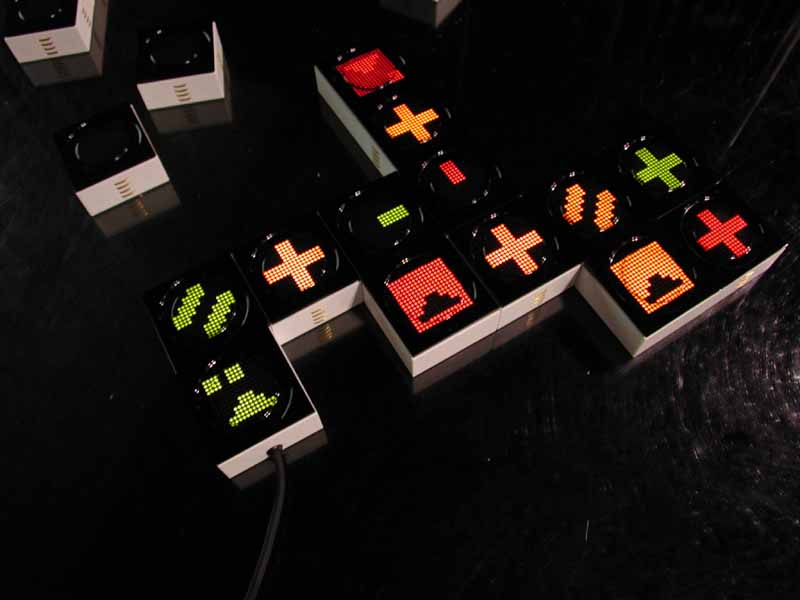
\includegraphics[width=12 cm]{images/blockjam.jpg}
  \centering
  \caption{Block Jam: music sequencer consist of a cluster of blocks}
  \label{fig: Block Jam}
\end{figure}
\bigskip

\section{Research goals and motivation}

While musical interfaces have been studied for a long time, there have emerged thousands of novel twists on \textquotedblleft{grid-based}\textquotedblright music sequencer. And to our knowledge there is currently no paper investigate the situation of this certain kind of musical application on App Store. What's more, there is no consensus on using what's method to evaluate those newborn musical application on mobile devices. This work is a first attempt to classify the music sequencers on iPad and adopt the evaluation method(MPX-Q Questionnaire) designed for NIME community. This work is guided by the following goals:
\begin{flushleft}
$\bullet$ Create an interface taxonomy of current music sequencer apps on the iOS app store.\\
$\bullet$ Perform a HCI user study to measure user experience and musicians performance with different interface design approaches.\\
$\bullet$ Propose design guidlines for musicians, developers and researcher for creating musical interface in the future.
\end{flushleft}
\section{Structure}

In the next chapter, literature relevant to the research topic was introduced, so as to establish a theoretical framework of the research (see Chapter \ref{ch: chapter 2}). And the research project was divided into two consecutive studies. In the first study, we analyzed the music sequencer applications (designed for iPad) on App Store and create an interface taxonomy (see Chapter \ref{ch: chapter 3}). Then base on the classification of music sequencer interfaces, we selected one most representative application from each category and conducted an user study to evlauate the effect of different interface design (see Chapter \ref{ch: chapter 4}). In Chapter \ref{ch: chapter 5}, we discussed the results and provided a conclusion of the study as well as the future work.
